\documentclass[12pt,a4paper]{article}
\usepackage[x11names]{xcolor}
\usepackage[T1]{fontenc}
\usepackage{xltxtra}
\usepackage{xunicode}

%\usepackage[top=1.2in,bottom=1.2in,left=1.2in,right=1in]{geometry} % 页边距
\defaultfontfeatures{Mapping=tex-text}%连字号

\usepackage[boldfont,slantfont,CJKchecksingle]{xeCJK} % 允许斜体和粗体
\xeCJKsetup{PunctStyle=hangmobanjiao}
\punctstyle{kaiming}
\setlength{\parindent}{0cm} 				% Default is 15pt.
\linespread{1.2}                       % 行间距
\setlength{\parskip}{\baselineskip}    % 段间距

\XeTeXlinebreaklocale "zh"
\XeTeXlinebreakskip = 0pt plus 1pt minus 0.1pt

\usepackage[unicode=true,colorlinks,linkcolor=blue]{hyperref} % 超链接
\setCJKmainfont[BoldFont=Lantinghei SC Demibold]{Heiti SC Light}
\setCJKmonofont{Menlo}
\setmainfont[BoldFont=Myriad Pro Bold, ItalicFont=Myriad Pro Italic]{Myriad Pro}
\setmonofont{Menlo}
\setsansfont{Arial}

\usepackage{graphicx}                   % 嵌入png图像
\usepackage{longtable,tabu,booktabs}
\usepackage{pdflscape}

\usepackage{tocloft}                        % 目录
\renewcommand\contentsname{目录}
\renewcommand{\today}{\number\year 年 \number\month 月 \number\day 日} % 中文日期

\usepackage{amsmath}
\numberwithin{equation}{section}

\usepackage{amsthm}

\theoremstyle{plain}
\newtheorem{thm}{定理}[section] % reset theorem numbering for each chapter

\theoremstyle{definition}
\newtheorem{defn}[thm]{定义} % definition numbers are dependent on theorem numbers
\newtheorem{exmp}[thm]{示例} % same for example numbers

\usepackage[linecolor=red,bordercolor=red,backgroundcolor=white,textwidth=5em,textsize=footnotesize]{todonotes}

\newcommand\abs[1]{\left|#1\right|}

\begin{document}

\title{\textbf{全彩屏校正软件设计}}

\author{卿培\\
        qingpei@sansitech.com
}

\date{\today}

\maketitle
\clearpage

\tableofcontents
\clearpage
\listoftodos

% !TEX root = ../The Design of Display Calibration Tool.tex

\section{设计总览} % (fold)
\label{sec:overview}

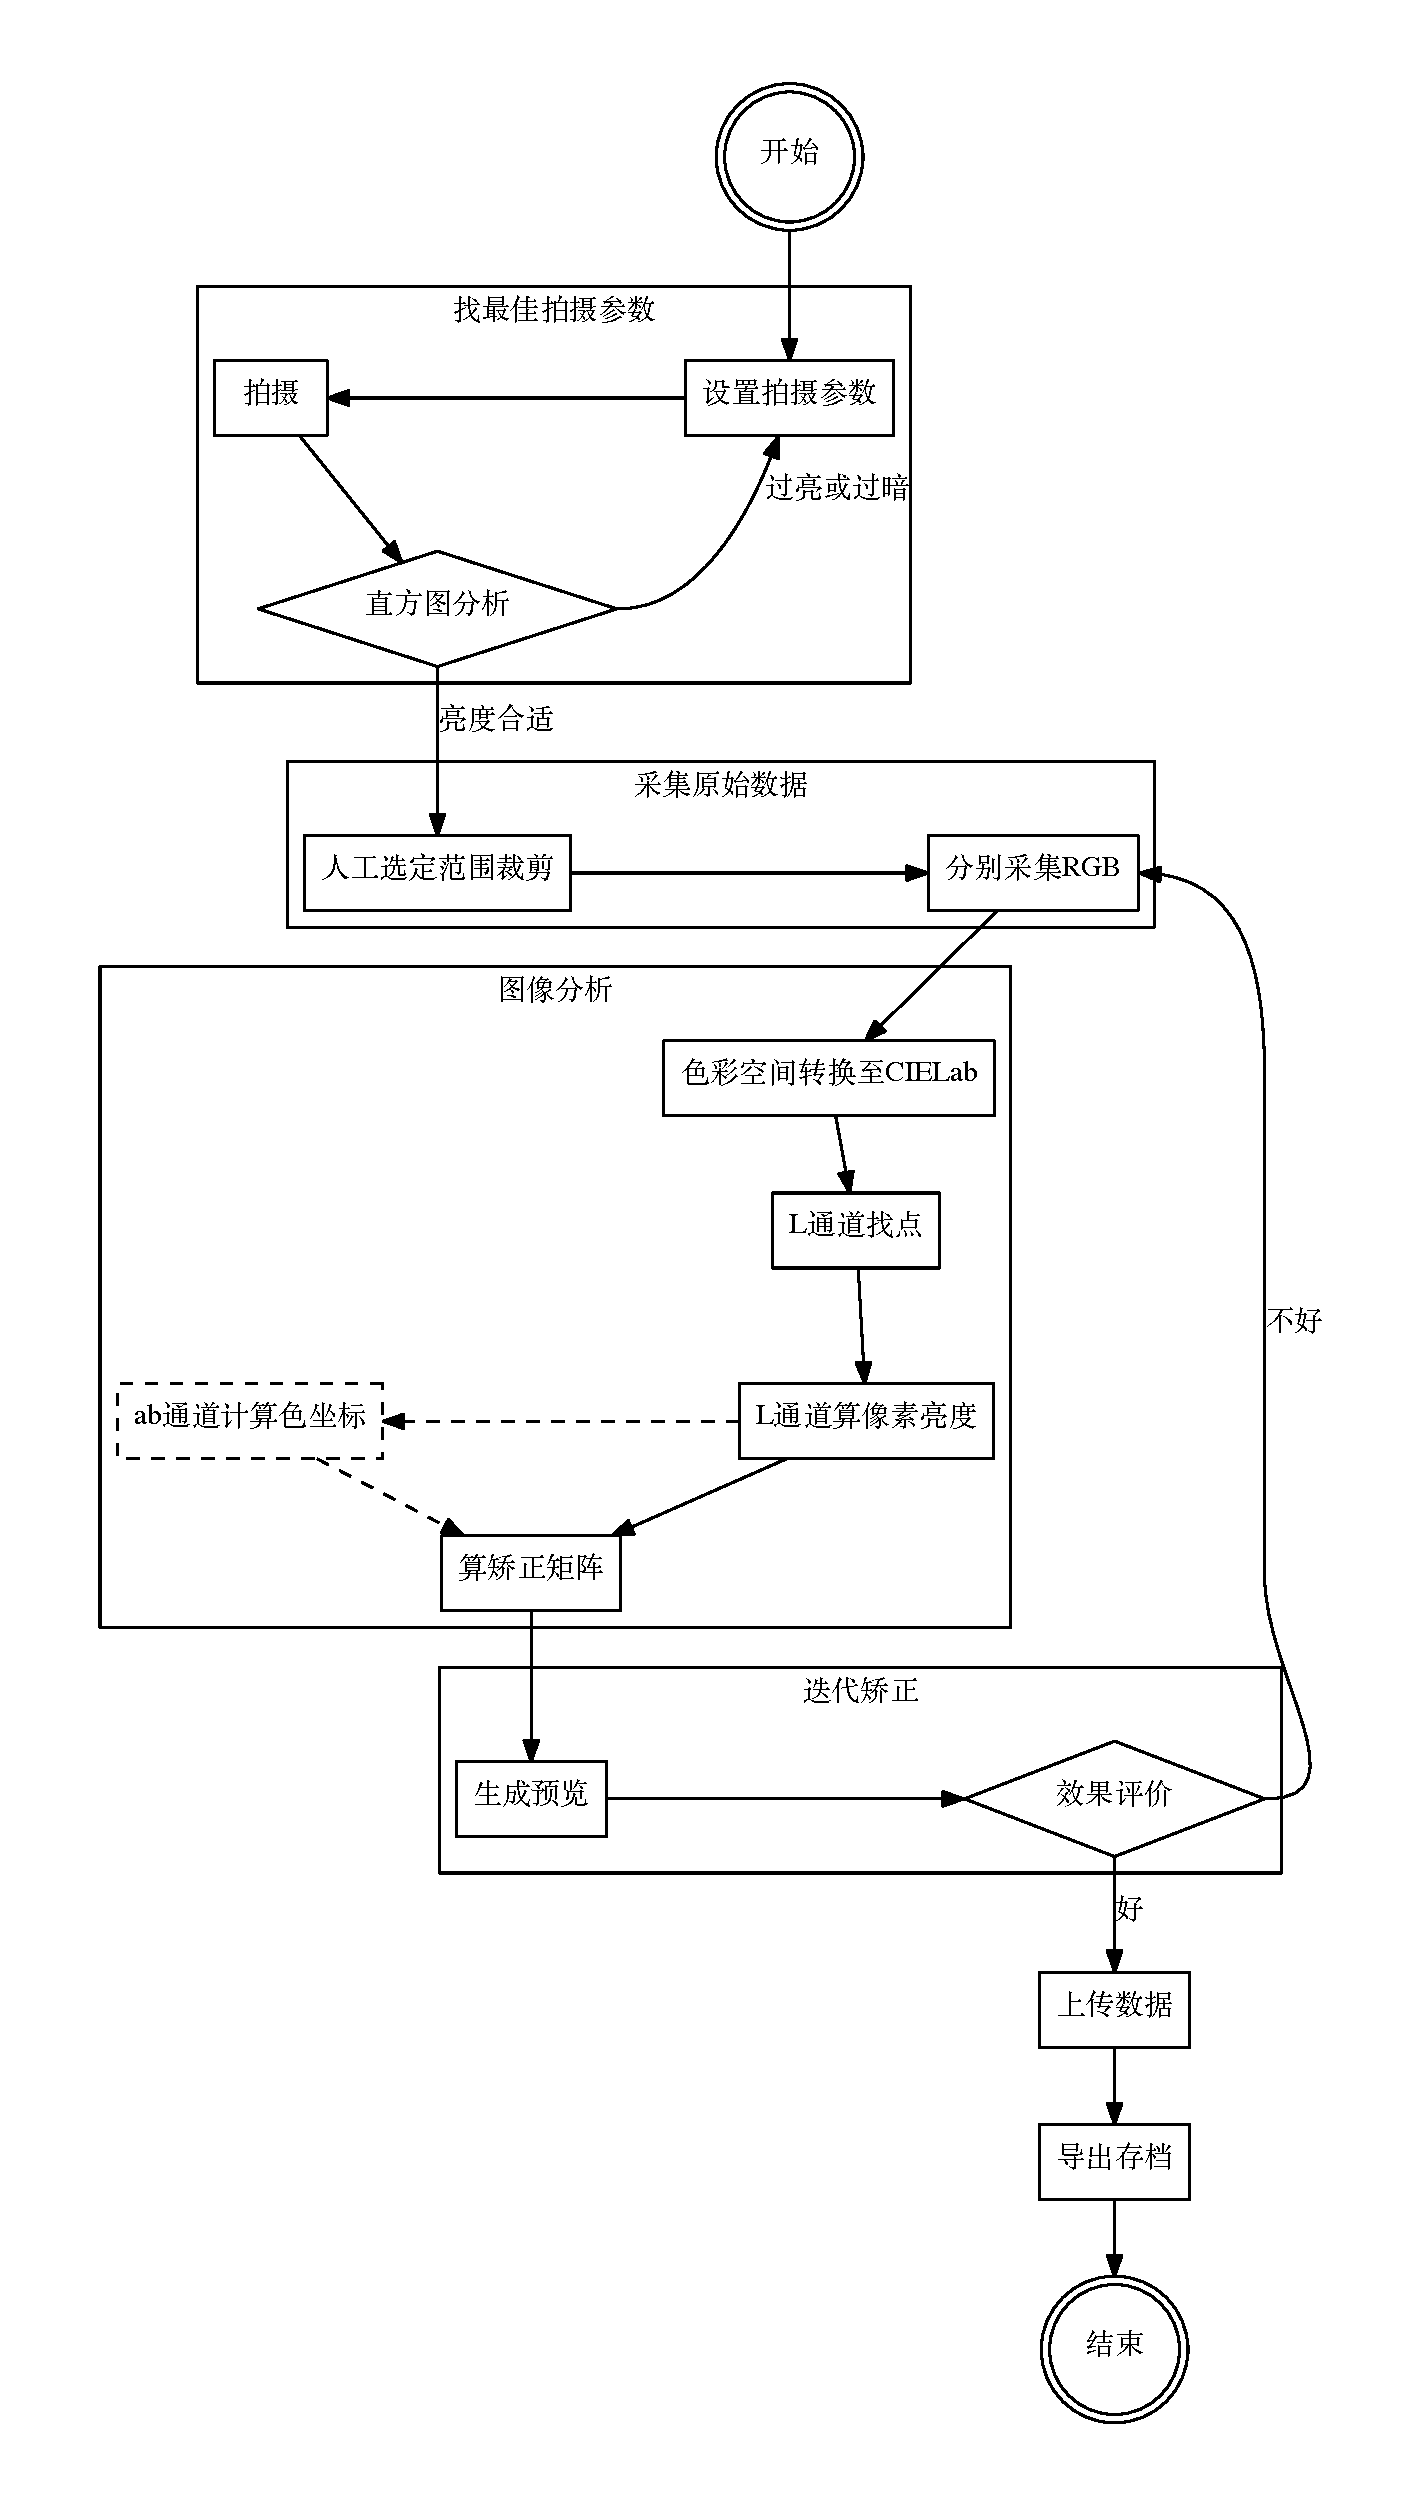
\includegraphics[height=\textheight]{calibration-process.pdf}

% section 设计总览(end)
% !TEX root = ../The Design of Display Calibration Tool.tex

\section{找最佳拍摄参数} % (fold)
\label{sec:configure}

焦距需要手动在镜头上调整,目标是被拍摄的屏幕范围应尽可能充满取景框。这里所寻找的参数是光圈快门组合。ISO应使用相机允许的最低值,以尽量避免噪点的产生。

寻找最优拍摄的步骤如下:

\begin{enumerate}
	\item 根据经验,预置一个默认参数
	\item 屏幕显示纯色,根据校正目标亮度调整,例如校正目标是50\%亮度下均匀,则使用 (127,127,127)
	\item \label{item:cap} 采集一张图像,分析灰度直方图
	\item 若饱和像素超过 1\% 的总像素,降低亮度,回到 \ref{item:cap}
	\item 亮度中位数在 200 以下,提高亮度,回到 \ref{item:cap}
	\item 饱和像素比例低于 1\%,且亮度中位数大于 200,完成\footnote{这几个步骤里的具体数值需要实际拍摄后确定,这里的数字仅为举例}
\end{enumerate}

在界面上应允许如下操作

\begin{enumerate}
	\item 人工设定参数
	\item 跳过参数设置
\end{enumerate}

人工设定参数的选项从相机读取可用的光圈、快门之后给出。

% section 找最佳拍摄参数 (end)

\section{图像采集} % (fold)
\label{sec:capture}

待整理。

% section 图像采集 (end)

% !TEX root = ../The Design of Display Calibration Tool.tex

\section{图像分析} % (fold)
\label{sec:analyze}

\subsection{色彩空间} % (fold)
\label{sub:colorspace}

RGB空间不宜进行亮度分析。三个通道皆对亮度有影响,容易顾此失彼。

CIELab 空间的提出就是为了解决此前色彩空间不能很好地反映肉眼感知的亮度。所以需要把采集的图像全部转换到此空间,用 L 通道的数据进行亮度矫正,(将来)用 ab 通道的数据进行色度矫正。

需要 $RGB \Leftrightarrow CIELab$ 的双向转换方法。

% subsection 色彩空间 (end)

\subsection{找点} % (fold)
\label{sub:findpixel}

使用 Hough Circles Transform 搜索图像中的发光单元,并确定每个单元的坐标、半径。

% subsection 找点 (end)

\subsection{显示质量评价} % (fold)
\label{sub:evaluation}

目前我们关注两个方面的显示质量:\emph{亮度均匀性}和\emph{色彩准确度}。

\subsubsection{亮度均匀性} % (fold)
\label{ssub:luminance_uniformity}

\begin{defn}
    全彩屏上一个像素$P$的\emph{亮度}$L_P$由采集到的照片中该像素范围内各个像素$p_i$在CIELAB空间$L$通道的几何平均值\footnote{相比于算术平均,几何平均对少量噪点更不敏感。}表示。

    \begin{equation}
        L_P = \left(\prod_{p_i \in P} L_{p_i} \right)^{1/n}
    \end{equation}
\end{defn}

\begin{defn}
    全彩屏的亮度均匀性为其中最大亮度像素与最小亮度像素的亮度比。

    \begin{equation}
        Luminance\ uniformity = \frac{L_{max}}{L_{min}}
    \end{equation}
\end{defn}

理想的亮度均匀性为$1$。这个比值越大,表示亮度均匀性越差。

这时需要一个检验标准来判定亮度均匀性是否合格,这个标准可以是$1.1$,可以是$1.3$,当然也可以是$1.05$等很严格的数值。\todo{了解这方面的现有标准}

另外一种评价方式是基于区域的。将一个显示屏分为$N$个区域,每个区域求出各自的平均亮度$L_i$,所有区域有一个全局的平均亮度$L_{avg}$,此时给出一个评价标准$\delta$,要求各个区域都符合标准。

\begin{equation}
    \abs{L_i - L_{avg}} < \delta
\end{equation}

同样,这里的$\delta$如何取值与上文一样需要商榷。

% subsubsection 亮度均匀性 (end)

\subsubsection{色彩准确度} % (fold)
\label{ssub:color_accuracy}

\begin{defn}
    全彩屏上一个像素$P_i$的颜色$(L_{P_i},a_{P_i},b_{P_i})$为采集到的照片中该像素范围内各个像素$p_j$在CIELAB空间$L,a,b$通道上的几何平均值。
\end{defn}

\begin{defn}
    全彩屏上一个像素$P_i$显示某个参考色时的\emph{色差}$\Delta E_{P_i,color}$为该像素的颜色与参考色的颜色由CIE DE2000\footnote{CIE DE2000很复杂,如果放宽要求可以采用CIE94甚至CIE76定义的色差。}定义的色差。

\end{defn}

理想情况下色差为$0$,数值越大表示偏色越严重。

\begin{defn}
    全彩屏的色彩准确度分为两项,一是平均色差$\Delta E_{avg,color}$,二是最大色差$\Delta E_{max,color}$。

    \begin{equation}
        \Delta E_{avg,color} = \frac{\sum_{i=1}^N{\Delta E_{P_i,color}}}{N}
    \end{equation}
    \begin{equation}
        \Delta E_{max,color} = max\left(\sum{\Delta E_{P,color}}\right)
    \end{equation}
\end{defn}

理想情况下色差为$0$。一般来说$\Delta E<2.3$属于被认为肉眼不可见。优化目标选择平均色差还是最大色差有待商榷。\todo{优化目标的选择也需要查一查显示器生产厂家是如何做的。}

% subsubsection 色彩准确度 (end)

% subsection 显示质量评价 (end)

% section 图像分析(end)
% \section{显示质量评价} % (fold)
\label{sec:evaluation}

目前我们关注两个方面的显示质量:\emph{亮度均匀性}和\emph{色彩准确度}。

\subsection{亮度均匀性} % (fold)
\label{sub:luminance_uniformity}

\begin{defn}
    全彩屏上一个像素$P$的\emph{亮度}$L_P$由采集到的照片中该像素范围内各个像素$p_i$在CIELAB空间$L$通道的几何平均值\footnote{相比于算术平均,几何平均对少量噪点更不敏感。}表示。

    \begin{equation}
        L_P = \left(\prod_{p_i \in P} L_{p_i} \right)^{1/n}
    \end{equation}
\end{defn}

\begin{defn}
    全彩屏的亮度均匀性为其中最大亮度像素与最小亮度像素的亮度比。

    \begin{equation}
        Luminance\ uniformity = \frac{L_{max}}{L_{min}}
    \end{equation}
\end{defn}

理想的亮度均匀性为$1$。这个比值越大,表示亮度均匀性越差。

这时需要一个检验标准来判定亮度均匀性是否合格,这个标准可以是$1.1$,可以是$1.3$,当然也可以是$1.05$等很严格的数值。\todo{了解这方面的现有标准}

另外一种评价方式是基于区域的。将一个显示屏分为$N$个区域,每个区域求出各自的平均亮度$L_i$,所有区域有一个全局的平均亮度$L_{avg}$,此时给出一个评价标准$\delta$,要求各个区域都符合标准。

\begin{equation}
    \abs{L_i - L_{avg}} < \delta
\end{equation}

同样,这里的$\delta$如何取值与上文一样需要商榷。

% subsection 亮度均匀性 (end)

\subsection{色彩准确度} % (fold)
\label{sub:color_accuracy}

\begin{defn}
    全彩屏上一个像素$P_i$的颜色$(L_{P_i},a_{P_i},b_{P_i})$为采集到的照片中该像素范围内各个像素$p_j$在CIELAB空间$L,a,b$通道上的几何平均值。
\end{defn}

\begin{defn}
    全彩屏上一个像素$P_i$显示某个参考色时的\emph{色差}$\Delta E_{P_i,color}$为该像素的颜色与参考色的颜色由CIE DE2000\footnote{CIE DE2000很复杂,如果放宽要求可以采用CIE94甚至CIE76定义的色差。}定义的色差。

\end{defn}

理想情况下色差为$0$,数值越大表示偏色越严重。

\begin{defn}
    全彩屏的色彩准确度分为两项,一是平均色差$\Delta E_{avg,color}$,二是最大色差$\Delta E_{max,color}$。

    \begin{equation}
        \Delta E_{avg,color} = \frac{\sum_{i=1}^N{\Delta E_{P_i,color}}}{N}
    \end{equation}
    \begin{equation}
        \Delta E_{max,color} = max\left(\sum{\Delta E_{P,color}}\right)
    \end{equation}
\end{defn}

理想情况下色差为$0$。一般来说$\Delta E<2.3$属于被认为肉眼不可见。优化目标选择平均色差还是最大色差有待商榷。\todo{优化目标的选择也需要查一查显示器生产厂家是如何做的。}

% subsection 色彩准确度 (end)

% section 显示质量评价 (end)

\section{亮度校正} % (fold)
\label{sec:correction}

经过亮度均匀性评价,我们得到每个像素的亮度表示。由于HoughCircles搜索到的圆并非按顺序排列的,需要将其对应到行和列。

然后将亮度数据重排成矩阵形式 $B$。

对于亮度矩阵,我们可以得到一个全像素平均亮度 $L_{overall}$。此时可以求出一个校正矩阵 $C$ 使得

\begin{equation}
    C \times B = L_{overall} \cdot I
\end{equation}

将校正矩阵 $C$ 应用于传输给控制盒的输出信号,等价于在硬件端进行校正。假设我们发给屏的信号亮度为 $B_{orig}$,采集到屏实际输出是上文提到的 $B$,那么屏的输入输出转化矩阵即为 $K$,它满足 $B_{orig} \times K = B$。

由于矩阵乘法满足结合律,下式也同样成立:

\begin{equation}
    C \times B_{orig} \times K = C \times B = L_{overall} \cdot I
\end{equation}

这样就可以通过校正输入信号来预览校正结果了。

% section 亮度校正 (end)


\end{document}
